\documentclass[12pt,a4paper]{article}

% --- Idioma y codificacion ---
\usepackage[spanish]{babel}
\usepackage[utf8]{inputenc}
\usepackage[T1]{fontenc}
\usepackage{titlesec}
\titleformat{\section}
  {\normalfont\large\bfseries}
  {\thesection}{1em}{}
\titleformat{\subsection}
  {\normalfont\normalsize\bfseries}
  {\thesubsection}{1em}{}
\titlespacing*{\section}{0pt}{12pt}{6pt}
\titlespacing*{\subsection}{0pt}{10pt}{5pt}

% --- Margenes ---
\usepackage[a4paper,
  top=2.5cm,bottom=2.5cm,
  left=2.2cm,right=2.2cm,
  columnsep=0.7cm
]{geometry}

% --- Graficos, tablas y matematicas ---
\usepackage{graphicx}
\usepackage{float}
\usepackage{amsmath}
\usepackage{amssymb}
\usepackage{booktabs}
\usepackage{siunitx}
\usepackage{array}
\usepackage{multicol}

% --- Enlaces e indice ---
\usepackage[hidelinks]{hyperref}
\addto\captionsspanish{\renewcommand{\contentsname}{Índice}}

% --- Encabezados y pies ---
\usepackage{fancyhdr}
\pagestyle{fancy}
\fancyhf{}
\lhead{Transmisión de señales en fibra óptica}
\rhead{\leftmark}
\cfoot{\thepage}
\setlength{\headheight}{14.62pt}
\addtolength{\topmargin}{-0.12pt}

% --- Formato numerico ---
\sisetup{output-decimal-marker={,}, per-mode=symbol}

\let\cleardoublepage\clearpage
\raggedcolumns
\setlength{\parindent}{0pt}
\setlength{\parskip}{2pt}
\renewcommand{\arraystretch}{1.2}
\setlength{\emergencystretch}{3em}
\linespread{1.08}\selectfont
\setlength{\abovedisplayskip}{6pt}
\setlength{\belowdisplayskip}{6pt}
\setlength{\abovedisplayshortskip}{6pt}
\setlength{\belowdisplayshortskip}{6pt}
\setlength{\abovecaptionskip}{5pt}
\setlength{\belowcaptionskip}{2pt}
\setlength{\textfloatsep}{8pt}
\setlength{\floatsep}{8pt}
\setlength{\intextsep}{8pt}

\begin{document}

% =========================
% Portada
% =========================
\begin{titlepage}
  \centering
  \vspace*{2cm}
  {\LARGE \textbf{Transmisión de señales en fibra óptica}\par}
  \vspace{1cm}
  {\large Asignatura: Laboratorio de Electromagnetismo II\par}
  \vspace{0.5cm}
  {\large Autor: Luis López Nasser\par}
  {\large Fecha: \today\par}
  \vfill
  {\large Universidad UNIE\par}
\end{titlepage}

% =========================
% Índice
% =========================
\tableofcontents
\clearpage

% =========================
% Contenido
% =========================
\begin{multicols}{2}

\section{Introducción}

\subsection{Marco teórico}

La fibra óptica es una guía dieléctrica en la que la luz se confina en el núcleo gracias a la diferencia de índice de refracción entre núcleo ($n_1$) y revestimiento ($n_2$), con $n_1>n_2$. La condición física de guiado se deriva de la ley de Snell:
\begin{equation}
n_1\sin\theta_1 = n_2\sin\theta_2.
\label{eq:snell}
\end{equation}
Cuando la luz pasa de un medio más denso a otro menos denso, existe un ángulo crítico para el cual el rayo refractado sale rasante. A partir de ese límite se produce reflexión interna total:
\begin{equation}
\theta_c = \arcsin\left(\frac{n_2}{n_1}\right).
\label{eq:theta_crit}
\end{equation}
Este es el mecanismo que permite transportar potencia óptica a largas distancias.

Para fibras de índice escalonado, la apertura numérica (NA) cuantifica el cono angular de aceptación:
\begin{equation}
\mathrm{NA}=n_0\sin\theta_{\max}\approx\sqrt{n_1^2-n_2^2},
\label{eq:na}
\end{equation}
donde $n_0\approx 1$ en aire. Esta magnitud también determina, por reciprocidad óptica, la divergencia del haz a la salida de la fibra. La documentación técnica y docente consultada en línea coincide en esta formulación [F1, F2].

La potencia óptica en una fibra real se atenúa por absorción del material, dispersión y pérdidas de guiado. El modelo macroscópico habitual es exponencial:
\begin{equation}
P(z)=P(0)e^{-\alpha z},
\label{eq:att_exp}
\end{equation}
y en decibelios por unidad de longitud:
\begin{equation}
\alpha_{\mathrm{dB}}=\frac{10}{L}\log_{10}\left(\frac{P_{\mathrm{in}}}{P_{\mathrm{out}}}\right).
\label{eq:alpha_db}
\end{equation}
Los textos técnicos diferencian además entre \textit{macrobending} (curvaturas visibles de radio finito) y \textit{microbending} (deformaciones locales pequeñas), ambos con incremento de pérdida cuando el radio de curvatura disminuye [F3, F4, F6].

En este laboratorio no se mide potencia óptica directamente, sino tensión eléctrica a la salida del receptor. Bajo operación lineal del fotodetector y de la electrónica de acondicionamiento, se asume proporcionalidad local $V\propto P$, por lo que la atenuación del guion puede escribirse como:
\begin{equation}
A = 10\log_{10}\left(\frac{V_x}{V_0}\right).
\label{eq:atenuacion}
\end{equation}
La incertidumbre propagada para variables independientes es:
\begin{equation}
\delta A = \frac{10}{\ln 10}\sqrt{\left(\frac{\delta V_x}{V_x}\right)^2+\left(\frac{\delta V_0}{V_0}\right)^2 }.
\label{eq:deltaA}
\end{equation}

Para la separación entre terminales, el fenómeno dominante es la divergencia del haz en el hueco de aire. En un modelo geométrico coaxial simplificado, la eficiencia de acoplamiento disminuye con la separación, y por tanto la atenuación crece con $l$. En el rango medido, esta caída suele aproximarse bien por una recta en dB o por una ley exponencial en escala lineal [F5].

En la cadena de audio, el sistema implementa una modulación analógica de intensidad. De forma simplificada:
\begin{align}
I_{\mathrm{LED}}(t) &= I_{\mathrm{bias}} + k_{\mathrm{TX}}v_{\mathrm{mic}}(t),\\
i_{\mathrm{PD}}(t) &= R_{\lambda}P_{\mathrm{opt}}(t) + i_n(t),
\end{align}
donde $R_{\lambda}$ es la responsividad del fotodetector e $i_n$ representa contribuciones de ruido. Esta relación explica por qué la alineación óptica y el nivel de señal influyen en la inteligibilidad final.

\subsection{Objetivos}

Los objetivos de la práctica son medir la atenuación por curvatura al incrementar el número de vueltas de la fibra, medir la pérdida por separación longitudinal entre terminales, ajustar modelos sencillos a los datos (lineal en dB y exponencial en tensión) para cuantificar pendientes con incertidumbre, y describir técnicamente la cadena de conversión acústico--eléctrico--óptico--eléctrico--acústico.

\section{Materiales}

Se emplearon el panel TX analógico (ANAL.TX), el panel RX analógico (ANAL.RX), el módulo de potenciómetro (POT), el micrófono (MIC.AMP), el amplificador de baja frecuencia (LF.AMP), fibras ópticas, un cilindro de torsión, un calibre de separación y un multímetro digital.

Además de los materiales, se identificaron las incertidumbres tipo B necesarias para el cálculo de errores. Como no se dispone de la ficha metrológica de cada instrumento en el cuaderno, se toman resoluciones inferidas del formato de lectura registrado.

\begin{table}[H]
\centering
\caption{Incertidumbres tipo B empleadas en el análisis.}
\label{tab:incertidumbres}
\small
\begin{tabular}{p{0.34\columnwidth}p{0.22\columnwidth}p{0.30\columnwidth}}
\toprule
Magnitud & Resolución asumida & $\delta x = \frac{\text{resolución}}{2}$ \\
\midrule
Voltaje torsión $V$ & \SI{0.01}{V} & $\pm$\SI{0.005}{V} \\
Voltaje separación $V$ & 0,1 u.a. & $\pm$0,05 u.a. \\
Separación $l$ (calibre) & \SI{0.1}{mm} & $\pm$\SI{0.05}{mm} \\
\bottomrule
\end{tabular}
\end{table}

\section{Procedimiento experimental}

\subsection{Ensayo 1: atenuación por torsión}

Se configuró el transmisor con señal de entrada desde POT y con enlace óptico directo ANAL.TX $\to$ ANAL.RX. A continuación se midió el voltaje de referencia con la fibra lo más recta posible ($N=0$ vueltas). Después se incrementó el número de vueltas alrededor del cilindro auxiliar desde 1 hasta 5, manteniendo inalterado el resto del montaje, y se registró en cada caso el voltaje de salida del receptor.

\subsection{Ensayo 2: atenuación por separación}

Se alinearon coaxialmente los dos terminales de fibra en el calibre y se registraron medidas de tensión para separaciones entre \SI{1}{mm} y \SI{10}{mm}, con incrementos de \SI{1}{mm}. En la hoja de datos no quedó anotado el punto $l=0$ mm (contacto), por lo que ese valor no se utiliza como dato medido en el análisis.

\subsection{Ensayo 3: transmisión de audio}

Se sustituyó la entrada POT por MIC.AMP en el transmisor. La señal óptica recibida se reconvirtió eléctricamente y se amplificó con LF.AMP, verificando de manera cualitativa el funcionamiento de la cadena completa de conversión.

\section{Datos experimentales}

\subsection{Torsión de la fibra}

\begin{table}[H]
\centering
\caption{Datos directos de voltaje para torsión de fibra.}
\label{tab:raw_torsion}
\small
\begin{tabular}{ccc}
\toprule
$N$ (vueltas) & $V$ (V) & $\delta V$ (V) \\
\midrule
0 & 2,62 & 0,005 \\
1 & 1,83 & 0,005 \\
2 & 1,58 & 0,005 \\
3 & 1,43 & 0,005 \\
4 & 0,93 & 0,005 \\
5 & 0,80 & 0,005 \\
\bottomrule
\end{tabular}
\end{table}

\subsection{Separación entre terminales}

\begin{table}[H]
\centering
\caption{Datos directos de voltaje para separación entre terminales.}
\label{tab:raw_sep}
\small
\begin{tabular}{ccc}
\toprule
$l$ (mm) & $V$ (u.a.) & $\delta V$ (u.a.) \\
\midrule
0  & ---  & --- \\
1  & 30,7 & 0,05 \\
2  & 26,7 & 0,05 \\
3  & 24,4 & 0,05 \\
4  & 20,4 & 0,05 \\
5  & 18,0 & 0,05 \\
6  & 15,9 & 0,05 \\
7  & 14,5 & 0,05 \\
8  & 13,2 & 0,05 \\
9  & 12,1 & 0,05 \\
10 & 11,4 & 0,05 \\
\bottomrule
\end{tabular}
\end{table}

\section{Análisis y discusión de datos}

\subsection{Atenuación por torsión}

Con $V_0=2{,}62$ V en $N=0$, la atenuación y su incertidumbre se calcularon con \eqref{eq:atenuacion} y \eqref{eq:deltaA}.

\begin{table}[H]
\centering
\caption{Resultados de atenuación para torsión.}
\label{tab:att_torsion}
\small
\begin{tabular}{ccc}
\toprule
$N$ & $V \pm \delta V$ (V) & $A \pm \delta A$ (dB) \\
\midrule
0 & $2,62 \pm 0,005$ & $0,000 \pm 0,012$ \\
1 & $1,83 \pm 0,005$ & $-1,559 \pm 0,014$ \\
2 & $1,58 \pm 0,005$ & $-2,196 \pm 0,016$ \\
3 & $1,43 \pm 0,005$ & $-2,630 \pm 0,017$ \\
4 & $0,93 \pm 0,005$ & $-4,498 \pm 0,025$ \\
5 & $0,80 \pm 0,005$ & $-5,152 \pm 0,028$ \\
\bottomrule
\end{tabular}
\end{table}

El ajuste lineal de $A$ frente a $N$ es:
\begin{equation}
A(N)=(-1{,}000\pm0{,}091)N+(-0{,}172\pm0{,}276).
\label{eq:fit_torsion}
\end{equation}
El coeficiente de determinación asociado al ajuste es $R^2=0{,}968$. Por tanto, la pérdida media en el intervalo estudiado es cercana a \SI{1}{dB} por vuelta. El comportamiento es consistente con pérdidas por macrocurvatura descritas en la bibliografía técnica [F3, F4, F6].

\begin{figure}[H]
\centering
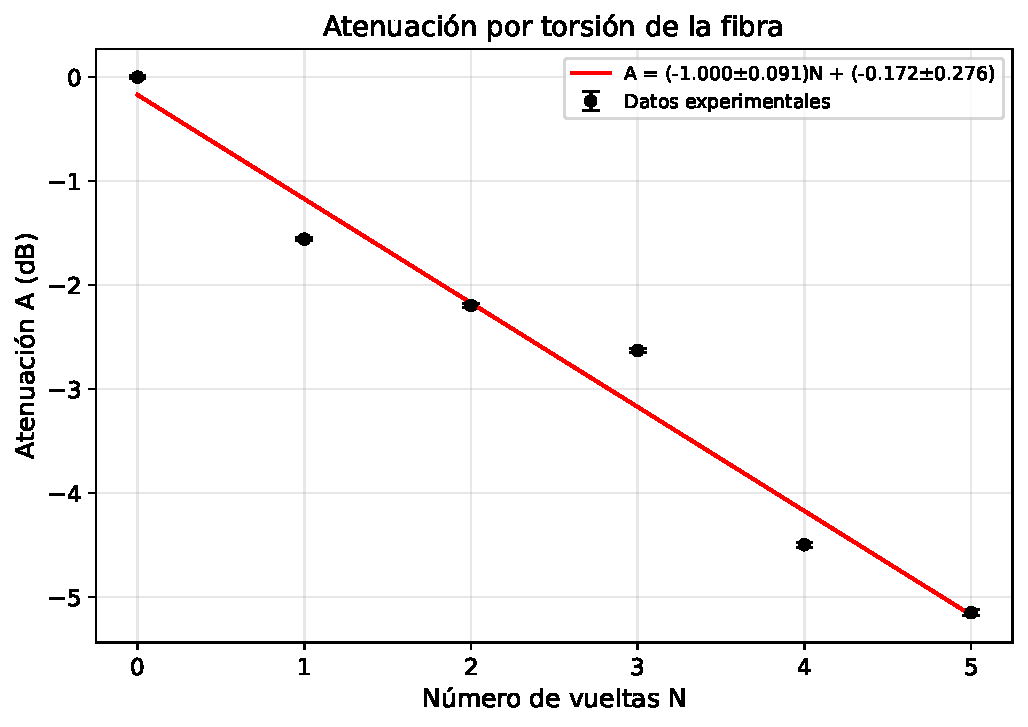
\includegraphics[width=1\columnwidth]{figuras/figura_1.pdf}
\caption{Atenuación de la señal en función del número de vueltas de torsión.}
\label{fig:figura1}
\end{figure}

\subsection{Atenuación por separación entre terminales}

Dado que no se registró el punto de referencia en $l=0$ mm, no se reporta atenuación absoluta $A=10\log(V/V_0)$ con dato medido. Para evitar introducir valores no medidos, el análisis principal se plantea de dos formas trazables:

\textbf{(i) Ajuste exponencial de la tensión medida.} Se ajusta:
\begin{equation}
\ln V(l)=kl+b.
\label{eq:lnfit_sep}
\end{equation}
Resultado experimental:
\begin{equation}
\ln V(l)=(-0{,}1132\pm0{,}0047)l + (3{,}498\pm0{,}029).
\label{eq:lnfit_sep_num}
\end{equation}
Con $R^2=0{,}987$.

\textbf{(ii) Atenuación relativa respecto a $l=1$ mm.} Se define
\begin{equation}
A_{\mathrm{rel}}(l)=10\log_{10}\left(\frac{V(l)}{V(1\,\mathrm{mm})}\right).
\label{eq:arel}
\end{equation}
Con propagación:
\begin{equation}
\delta A_{\mathrm{rel}} = \frac{10}{\ln 10}\sqrt{\left(\frac{\delta V(l)}{V(l)}\right)^2 + \left(\frac{\delta V_1}{V_1}\right)^2 }.
\label{eq:darel}
\end{equation}

\begin{table}[H]
\centering
\caption{Atenuación relativa por separación (referencia en $l=1$ mm).}
\label{tab:arel_sep}
\small
\begin{tabular}{ccc}
\toprule
$l$ (mm) & $V \pm \delta V$ (u.a.) & $A_{\mathrm{rel}} \pm \delta A_{\mathrm{rel}}$ (dB) \\
\midrule
1  & $30,7 \pm 0,05$ & $0,000 \pm 0,010$ \\
2  & $26,7 \pm 0,05$ & $-0,606 \pm 0,011$ \\
3  & $24,4 \pm 0,05$ & $-0,997 \pm 0,011$ \\
4  & $20,4 \pm 0,05$ & $-1,775 \pm 0,013$ \\
5  & $18,0 \pm 0,05$ & $-2,319 \pm 0,014$ \\
6  & $15,9 \pm 0,05$ & $-2,857 \pm 0,015$ \\
7  & $14,5 \pm 0,05$ & $-3,258 \pm 0,017$ \\
8  & $13,2 \pm 0,05$ & $-3,666 \pm 0,018$ \\
9  & $12,1 \pm 0,05$ & $-4,044 \pm 0,019$ \\
10 & $11,4 \pm 0,05$ & $-4,302 \pm 0,020$ \\
\bottomrule
\end{tabular}
\end{table}

El ajuste lineal de $A_{\mathrm{rel}}$ frente a $l$ es:
\begin{equation}
A_{\mathrm{rel}}(l)=(-0{,}492\pm0{,}020)l + (0{,}321\pm0{,}125).
\label{eq:fit_sep_rel}
\end{equation}
El ajuste presenta $R^2=0{,}987$.
La pendiente negativa muestra que la separación incrementa de forma sistemática la pérdida de acoplamiento, en acuerdo con el mecanismo de divergencia del haz en el hueco de aire [F5].

\begin{figure}[H]
\centering
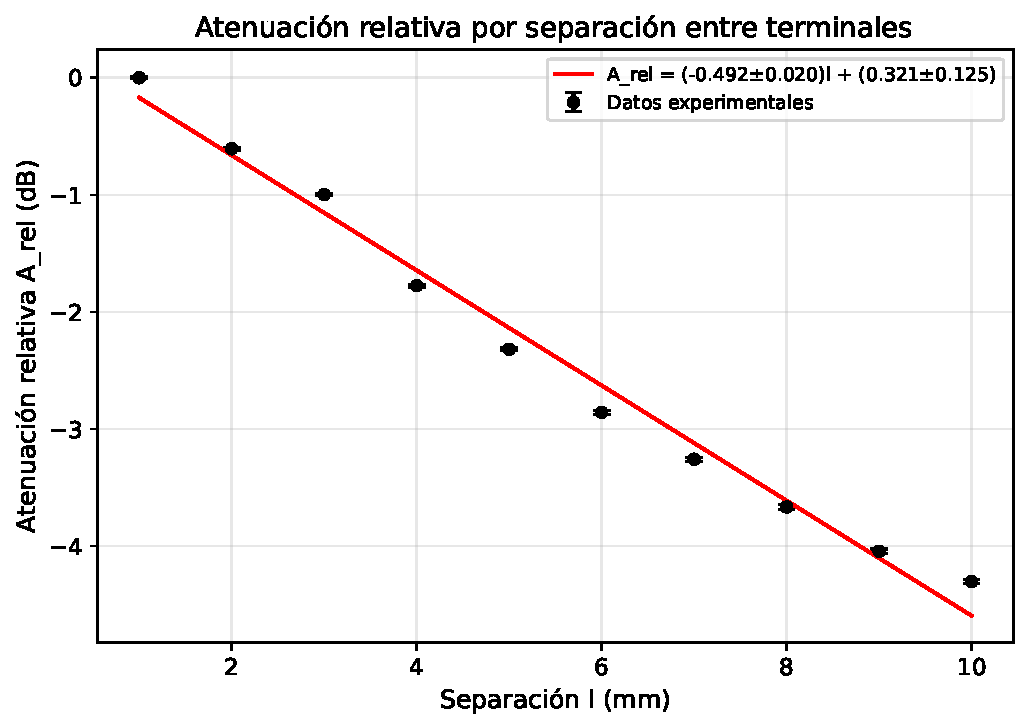
\includegraphics[width=1\columnwidth]{figuras/figura_2.pdf}
\caption{Atenuación relativa de la señal frente a la separación entre terminales.}
\label{fig:figura2}
\end{figure}

\subsection{Conversión acústica a óptica y recuperación}

En el material disponible no se incluyen anotaciones cualitativas detalladas de escucha (ruido, distorsión, inteligibilidad o estabilidad temporal). Para no introducir información no medida, se documenta únicamente el marco físico de interpretación:

Si la alineación óptica empeora, disminuye la potencia recibida y baja la relación señal/ruido en la salida de audio. Si el transmisor trabaja fuera de su zona lineal, pueden aparecer distorsiones por recorte o compresión en amplitud. En todo caso, el enlace verifica el principio de conversión en cascada acústico $\to$ eléctrico $\to$ óptico $\to$ eléctrico $\to$ acústico.

Con una próxima sesión de laboratorio, convendría registrar de forma explícita observaciones auditivas con una escala simple (nivel, claridad y ruido) para cerrar cuantitativamente esta parte.

\section{Conclusiones}

La atenuación por torsión aumenta de forma clara con el número de vueltas. En este montaje se obtiene una pendiente de $(-1{,}000\pm0{,}091)$ dB/vuelta y una pérdida acumulada de \SI{5.15}{dB} entre 0 y 5 vueltas. En separación de terminales, la tensión recibida sigue una caída exponencial con la distancia: $\ln V(l)=(-0{,}1132\pm0{,}0047)l+(3{,}498\pm0{,}029)$, con $R^2=0{,}987$. Como no se dispone de medida directa de $V_0$ en $l=0$ mm, no es correcto reportar atenuación absoluta basada en contacto; como alternativa trazable, la atenuación relativa respecto a $l=1$ mm da una pendiente de $(-0{,}492\pm0{,}020)$ dB/mm. Por último, la cadena de transmisión de audio queda descrita por el modelo de modulación de intensidad y detección fotoeléctrica, y para cerrar esta parte sin ambigüedad experimental faltan únicamente observaciones cualitativas registradas en cuaderno.

\section*{Fuentes en línea consultadas}

[F1] Thorlabs, \emph{The Fundamentals of Fiber Optics}, \href{https://www.thorlabs.us/newgrouppage9.cfm?objectgroup_id=14202}{enlace}. [F2] RP Photonics Encyclopedia, \emph{Numerical Aperture}, \href{https://www.rp-photonics.com/numerical_aperture.html}{enlace}. [F3] RP Photonics Encyclopedia, \emph{Bend Losses}, \href{https://www.rp-photonics.com/bend_losses.html}{enlace}. [F4] FOA, \emph{Microbending and Macrobending Fiber Losses}, \href{https://foa.org/tech/ref/fiber/Microbending.html}{enlace}. [F5] FOA, \emph{Loss and Optical Power Measurement}, \href{https://foa.org/tech/ref/testing/test/loss.html}{enlace}. [F6] ITU-T, \emph{Recommendation G.657 summary} (bend-insensitive optical fibre), \href{https://www.itu.int/dms_pubrec/itu-t/rec/g/T-REC-G.657-200911-S!!SUM-HTM-E.htm}{enlace}.

\end{multicols}

\end{document}
